\section{A twenty-bit witness and its consequences}
\label{sec:witness}

\subsection{The complete construction}

Split twenty independent signs into five blocks of four. Let
\(U,Z_1,Z_2,Z_3,Z_4\) be the corresponding raw block sums. Their
common distribution is
\begin{center}
\begin{tabular}{@{}rrrrrr@{}}
\toprule
\(t\)&\(-4\)&\(-2\)&\(0\)&\(2\)&\(4\)\\
\(16p(t)\)&1&4&6&4&1\\
\bottomrule
\end{tabular}
\end{center}
Their variance is four. Use the singleton targets
\[
 (a_1,a_2,a_3,a_4)=(-2,0,2,4)
\]
and the selector in the following exact table.
\begin{center}
\begin{tabular}{@{}rrrrrr@{}}
\toprule
Central sum \(t\)&\(-4\)&\(-2\)&\(0\)&\(2\)&\(4\)\\
Selected index \(\iota(t)\)&1&2&3&4&3\\
Selected target \(a_{\iota(t)}\)&\(-2\)&0&2&4&2\\
Ratio \(w_t\)&\(1/4\)&\(2/3\)&\(3/2\)&4&\(1/4\)\\
Mismatch \(t-a_{\iota(t)}\)&\(-2\)&\(-2\)&\(-2\)&\(-2\)&2\\
\bottomrule
\end{tabular}
\end{center}
Apply the report from Section~\ref{sec:reporter}. In this singleton
case the all-pass report \(B\) is itself just one tag.

\begin{theorem}[Exact twenty-bit certificate]\label{thm:witness}
The observation \(F_*\) just defined has 622 attained cells and
maximum cell degree exactly 16. Its retained variance is
\[
 v(F_*)=\frac{557065}{34816}
       =16+\frac9{34816}.
\]
The exceptional cell has probability \(17/2048\), cardinality 8704,
and conditional coordinate-sum law
\begin{center}
\begin{tabular}{@{}rrrrrrr@{}}
\toprule
\(h\)&\(-2\)&0&2&4&6&10\\
\(1088\,\Pbb(H_{20}=h\mid A)\)&77&296&417&248&47&3\\
\bottomrule
\end{tabular}
\end{center}
Consequently
\[
 \E[H_{20}\mid A]=\frac{31}{17},\qquad
 \E[H_{20}^2\mid A]=\frac{124}{17},\qquad
 \Var(H_{20}\mid A)=\frac{1147}{289}=4-\frac9{289}.
\]
\end{theorem}

\begin{proof}
Each block has four bits, so Proposition~\ref{prop:reporter} gives
degree at most 16 for every output. Let \(S\) be the set of all sixteen
leaf coordinates. In \eqref{eq:reporter-cancellation}, each term in
the sum omits one leaf block, and hence has zero coefficient on \(S\).
For the product of all four target indicators, the top character of
each block is constant on its target level. If the block sum is \(a\),
that constant is \((-1)^{(4-a)/2}\). The four exponents are
\(3,2,1,0\), whose sum is even. Thus
\[
 \widehat{\1_A}(S)
 =-\prod_{j=1}^4p(a_j)
 =-\frac3{2048}\ne0.
\]
This proves \(\deg\1_A=16\) and therefore \(D(F_*)=16\).

For each of the five central sums, there are \(5^3\) possibilities
for the unselected leaf sums. Exactly one is all-pass; the remaining
\(5^3-1=124\) produce distinct ordinary reports. Every such report
is attained. Adding the two special reports gives
\(5\cdot124+2=622\).

The table and \eqref{eq:singleton-parameters} give
\[
 Q=\frac3{2048},\quad
 W=\frac{20}{3},\quad K_0=\frac{17}{3},\quad
 a_\Sigma=4,\quad R_1=-\frac{37}{3},\quad H_2=\frac{80}{3}.
\]
Hence
\[
 \Pbb(A)=QK_0=\frac{17}{2048},\qquad
 b_*=4-\frac{37}{17}=\frac{31}{17}.
\]
Moreover,
\[
 \frac{R_1^2}{K_0}-H_2
 =\frac{1369}{51}-\frac{1360}{51}
 =\frac3{17}.
\]
Theorem~\ref{thm:finite-selector} gives the claimed retained variance.

For completeness the conditional law can be calculated directly,
independently of that formula. Given \(U=t\), put \(i=\iota(t)\).
For each \(z\ne a_i\), event
\[
 U=t,\quad Z_i=z,\quad Z_j=a_j\quad(j\ne i)
\]
has probability \(Qw_t p(z)\), and the total sum is
\(t+z+4-a_i\). Sum those finitely many contributions at each value of
the total. The resulting cardinalities are
\[
 (616,2368,3336,1984,376,24)
\]
at \((-2,0,2,4,6,10)\), respectively. Their sum is 8704, and division
by 8704 yields the displayed law. Its first two moments are
\(31/17\) and \(124/17\), whose variance is \(1147/289\).
All other cells retain an independent four-bit sum and hence have
conditional variance four. Equation~\eqref{eq:total-variance}
then gives the same global advantage directly:
\[
 v(F_*)-16=
 \frac{17}{2048}\left(4-\frac{1147}{289}\right)
 =\frac9{34816}.
\]
\end{proof}

\begin{figure}[tb]
\centering
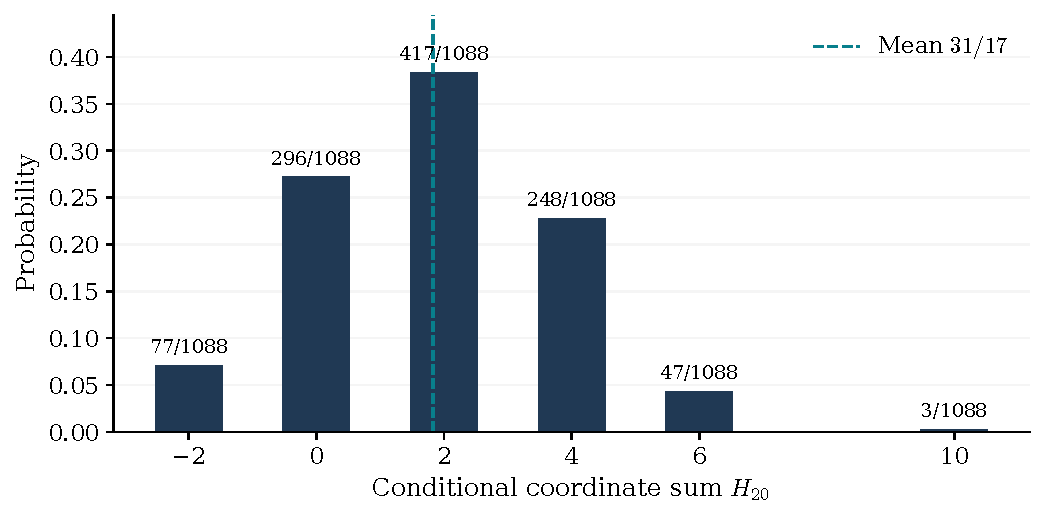
\includegraphics[width=.86\linewidth]{figures/exceptional_cell.pdf}
\caption{The exact conditional law on the exceptional twenty-bit cell.
The distribution is a law on six sums, with unequal spacings. Its
variance is \(1147/289<4\). The discrete probabilities, not a fitted
curve, determine the certificate.}
\label{fig:exceptional}
\end{figure}

Together with the codimension obstruction, Theorem~\ref{thm:witness}
proves Theorem~\ref{thm:headline}. It also shows why testing only
coordinate-subcube partitions would miss the phenomenon.

\subsection{The complete score law and its moments}

The four central values with mismatch \(-2\) have total ratio
\(77/12\); the remaining value has ratio \(1/4\).
Equation~\eqref{eq:finite-score-law} therefore simplifies to
\begin{equation}\label{eq:witness-score-law}
 \Law(T_{F_*})=\Law(H_{16})+
 \frac{-77\delta_2-3\delta_6+12\delta_4+68\delta_{31/17}}{8192}.
\end{equation}
This is a compact exact certificate for every score moment. For example,
\begin{align}
 \E T_{F_*}^3&=-\frac{6045}{591872},\notag\\
 \E T_{F_*}^4&=\frac{7403910529}{10061824}
             =736-\frac{1591935}{10061824},\label{eq:witness-moments}\\
 \kappa(F_*)&=\frac{15163208763392}{5275464041825}
             \simeq2.8742890944.\notag
\end{align}
Its moment generating function is the entire function
\begin{equation}\label{eq:witness-mgf}
 \E e^{tT_{F_*}}
 =(\cosh t)^{16}+
 \frac{-77e^{2t}-3e^{6t}+12e^{4t}+68e^{31t/17}}{8192}.
\end{equation}

\begin{lemma}[Symmetrizing an observation]\label{lem:symmetrize}
Let \(F\) be an observation of \(N\) bits with score \(T\), degree
\(D\), and variance \(v\). Introduce an independent sign \(z\), put
\(x'=zx\) coordinatewise, and report
\[
 F^{\mathrm{sym}}(z,x)=(z,F(x')).
\]
This is an observation of \(N+1\) bits with cell degree at most \(D+1\).
Its score is \(z(1+T)\), where \(z\) and \(T\) are independent, so
its law is symmetric and its retained variance is \(v+1\).
\end{lemma}

\begin{proof}
The change of variables \((z,x)\mapsto(z,x')\) preserves the uniform
product law. The full coordinate sum becomes \(z(1+H_N(x'))\);
conditioning gives the displayed score.
For each Walsh monomial in a cell indicator,
substitution produces \(z^{|S|}\chi_S(x)\).
Multiplication by \(\1_{\{z=\varepsilon\}}=(1+\varepsilon z)/2\)
has degree at most \(|S|+1\), proving the bound. Finally
\(\E(1+T)^2=1+v\).
\end{proof}

For our witness the symmetrized score has moment generating function
\[
 (\cosh t)^{17}
 +\frac{-77\cosh(3t)-3\cosh(7t)
       +12\cosh(5t)+68\cosh(48t/17)}{8192}.
\]
Its variance is \(591881/34816\) and its fourth moment is
\(8379512003/10061824\). Yet its first absolute moment is exactly
the seventeen-bit majority benchmark:
\begin{equation}\label{eq:oddified-benchmark}
 \E|z(1+T_{F_*})|=B_{17}.
\end{equation}
Indeed the correction to the first absolute moment is
\[
 \frac{-77\cdot3-3\cdot7+12\cdot5+68(48/17)}{8192}=0,
\]
and \(\E|1+H_{16}|=\E|H_{17}|\) by symmetry.
Likewise the correction to \(\E|T_{F_*}|\) in
\eqref{eq:witness-score-law} is zero, giving \(B_{16}\).
The exact degree of \(f=\sgn(T_{F_*})\) is 16. One certificate is
the coefficient \(165/16384\) on the set consisting of all four
central coordinates and all coordinates of leaf blocks 2, 3, and 4;
the verification script computes it by integer summation.
All possible scores are even integers or \(31/17\), so
\(\sgn(1+T_{F_*})=\sgn(T_{F_*})\). The symmetrized readout is therefore
\(z f(zx)\). The same nonzero degree-16 coefficient becomes a
degree-17 coefficient after multiplication by \(z\), proving its
exact degree is 17.
Thus these particular readouts have singleton sums \(B_{16}<\sqrt{16}\)
and \(B_{17}<\sqrt{17}\), respectively. The finite variance advantage
does not itself give a Boolean square-root counterexample.

\subsection{Tensorization, padding, and an extremal function}

\begin{definition}
For integers \(0\le D\le N\), let
\[
 V(N,D)=\max\{v(F):F\text{ is an observation of }N\text{ bits},
                  \ D(F)\le D\}.
\]
The maximum exists because a finite set has only finitely many
partitions; labels do not affect the value.
\end{definition}

\begin{theorem}[A global exact lower bound]\label{thm:tensor}
Put
\[
 q=\min\left\{\left\lfloor\frac D{16}\right\rfloor,
               \left\lfloor\frac{N-D}{4}\right\rfloor\right\}.
\]
Then
\begin{equation}\label{eq:extremal-lower}
 V(N,D)\ge D+\frac9{34816}q.
\end{equation}
If \(N-D\in\{0,1,2,3\}\), then \(V(N,D)=D\).
For every \(k\ge4\) and \(N\ge k+16\), there is an observation
of exact degree \(N-k\) with retained variance
\(N-k+9/34816\).
\end{theorem}

\begin{proof}
Take \(q\) disjoint copies of \(F_*\), reveal a further
\(r=D-16q\) individual signs, and ignore
\(s=N-D-4q\) signs. Both \(r\) and \(s\) are nonnegative integers,
and \(20q+r+s=N\). Lemma~\ref{lem:observation-calculus} gives exact
degree \(16q+r=D\) and variance
\(q(16+9/34816)+r\).
This proves \eqref{eq:extremal-lower}.
For deficits one through three the matching upper bound is the
codimension theorem; deficit zero uses \(v(F)\le N\).
For the final assertion use one copy, \(N-k-16\) revealed signs,
and \(k-4\) ignored signs.
\end{proof}

In particular, for \(q\ge1\),
\[
 V(20q,16q)\ge16q\left(1+\frac9{557056}\right).
\]
Thus no constant \(C\) can make \(v(F)\le D(F)+C\) hold for all
observations. At the single-cell level, the product cell \(A^q\) has
degree \(16q\) and conditional variance
\(4q-9q/289\). Tensorization makes the additive defect unbounded,
but leaves the ratio from this fixed witness unchanged. Improving
that ratio without bound requires a further mechanism, such as the
uniform amplifier below.

\begin{corollary}[A strict bound at codimension four]
\label{cor:strict-four}
For \(N\ge4\), every nonempty cell with
\(\deg\1_C\le N-4\) satisfies \(\Var(H_N\mid C)>3\).
Consequently
\[
 V(N,N-4)<N-3.
\]
\end{corollary}

\begin{proof}
The degree assumption gives the four alternating cancellations for
\(Y=(N-H_N)/2\). Proposition~\ref{codim:four-relaxation}
gives \(\Var(Y)>3/4\), proving the cellwise assertion.
Its positive-weight average gives \(v(F)<N-3\).
There are finitely many partitions of the \(N\)-cube, so the
maximum defining \(V(N,N-4)\) also satisfies the strict inequality.
\end{proof}

\subsection{An asymptotic retention profile}

\begin{proposition}[Existence and concavity of the profile]
\label{prop:profile}
For every \(0\le\rho\le1\), the limit
\[
 \Phi(\rho)=\lim_{N\to\infty}
        \frac{V(N,\lfloor\rho N\rfloor)}N
 =\sup_{N\ge1}\frac{V(N,\lfloor\rho N\rfloor)}N
\]
exists. The function is nondecreasing and concave, with
\(\Phi(0)=0\), \(\Phi(1)=1\), and
\begin{equation}\label{eq:profile-lower}
 \Phi(\rho)\ge\rho+\frac9{34816}
       \min\left\{\frac{\rho}{16},\frac{1-\rho}{4}\right\}.
\end{equation}
In particular \(\Phi(\rho)>\rho\) for every \(0<\rho<1\).
\end{proposition}

\begin{proof}
Tensorization gives
\[
 V(N_1+N_2,D_1+D_2)\ge V(N_1,D_1)+V(N_2,D_2).
\]
The degree budget is monotone, and
\(\lfloor\rho N_1\rfloor+\lfloor\rho N_2\rfloor
\le\lfloor\rho(N_1+N_2)\rfloor\).
Thus \(a_N=V(N,\lfloor\rho N\rfloor)\) is superadditive and
bounded above by \(N\). For completeness, fix \(r\) and write
\(N=qr+s\), \(0\le s<r\). Superadditivity and nonnegativity give
\(a_N\ge q a_r\); therefore
\(\liminf_Na_N/N\ge a_r/r\). Taking the supremum over \(r\)
proves existence and the displayed supremum formula.

Monotonicity follows directly from the degree budget. For concavity,
let \(\rho_1\ge\rho_2\), \(0<t<1\), and
\(\rho=t\rho_1+(1-t)\rho_2\).
Set \(N_1=\lfloor tN\rfloor\), \(N_2=N-N_1\). Then
\[
 \lfloor\rho_1N_1\rfloor+\lfloor\rho_2N_2\rfloor
 \le\left\lfloor\rho_2N+(\rho_1-\rho_2)N_1\right\rfloor
 \le\lfloor\rho N\rfloor.
\]
The product lower bound, divided by \(N\) and passed to the limit,
proves
\(\Phi(\rho)\ge t\Phi(\rho_1)+(1-t)\Phi(\rho_2)\).
The endpoint values follow from constant observations and full
revelation. Finally divide \eqref{eq:extremal-lower} by \(N\)
with \(D=\lfloor\rho N\rfloor\), and pass to the limit.
\end{proof}
